\documentclass[a4paper]{article}

\usepackage{babel}
\usepackage[latin1]{inputenc}
\usepackage{amssymb}
\usepackage{framed}
\usepackage{graphicx}

\setlength{\parindent}{0pt}
\setlength{\parskip}{3ex}

\begin{document}

\begin{center}
  {\large Artificial Neural Networks and Deep Architectures, DD2437}\\
  \vspace{7mm}
  {\huge Short report on lab assignment 2\\[1ex]}
  {\Large Radial basis functions, competitive learning and self-organisation}\\
  \vspace{8mm}  
  {\Large Rakin Ali, Steinar Logi and Hasan \textbf{Efternamn}\\}
  \vspace{4mm}
  {\large January,08 2023\\}
\end{center}

\section{Main objectives and scope of the assignment}

Our major goals in the assignment were  
\begin{itemize}
\item To build, design and analyze a RBF network 
\item To understand Vector Quantization and how to implement it  
\item To implement Self organising maps in order to understand the underlying theory behind it
\end{itemize}

\section{Methods} All parts of the labs were implemented twice just to be safe. Everything was written in Python 3.9 and all plots were done with Matplotlib. 

\section{Results and discussion - Part I: RBF networks and Competitive Learning \normalsize{\textit{(ca. 2.5-3 pages)}}}


\subsection{Function approximation with RBF networks\\ \normalsize{\textit{(ca. 1.5-2 pages)}}}
\textit{Combine results and findings from RBF simulations on both noise-free and noisy function approximation (sin(2x) and square (2x)). Try to organise them into subsections, and please make sure you pay attention to the comparison between RBF- and MLP-based approaches as well as the comparative analyses of batch and on-line learning schemes. Answer the questions, quantify the outcomes, discuss your interpretations and summarise key findings as conclusions.}


We performed function approximation with Radial basis function networks. The functions we approximated were the $sin(2x)$ and $square(2x)$ functions. The training set for the functions was obtained by using the domain $[0:2\pi]$. The step size was 0.1 and we sampled both the functions to obtain the training set. For the test set we started from 0.05 and used the same step size. The networks were trained using batch mode. The two function that we approximated can be seen in figure \ref{fig:two-functions}\\

\begin{figure}
    \centering
    \includegraphics{}
    \caption{Caption}
    \label{fig:enter-label}
\end{figure}

When fitting the radial basis function network to the sine function we discovered that it was enough to use only 4 units to be able to obtain an error below 0.1 and to obtain an error below 0.01 it was enough to use 6 units. When using 4 units we placed them at each minimum and maximum of the sine wave in the interval $[0:2\pi]$. When we used 6 neurons we placed the units at each minimum and maximum and then we placed two neurons at the ends of the interval. \\

When we fitted the $square(2x)$ function we observed that if we used the $sgn(y)$ activation function in the output layer we could reduce the error to zero. The $sgn(y)$ returns 1 if the input, $y$, is greater or equal to zero and -1 if the input is less than zero. The width of the radial basis functions was 2. This approximated function can be seen in figure \ref{fig:square-non} 



\subsection{Function approximation with noise data}
In t

\subsection{Competitive learning for RBF unit initialisation\\ \normalsize{\textit{(ca. 1 page)}}}
\textit{Please refer first to the results in the previous section, i.e. those obtained without any automated initialisation. Then in the next subsection focus on two-dimensional regression with RBF networks.}


\section{Results and discussion - Part II: Self-organising maps \normalsize{\textit{(ca. 2 pages)}}}

\subsection{Topological ordering of animal species}
\begin{figure} [htb]
    \centering
    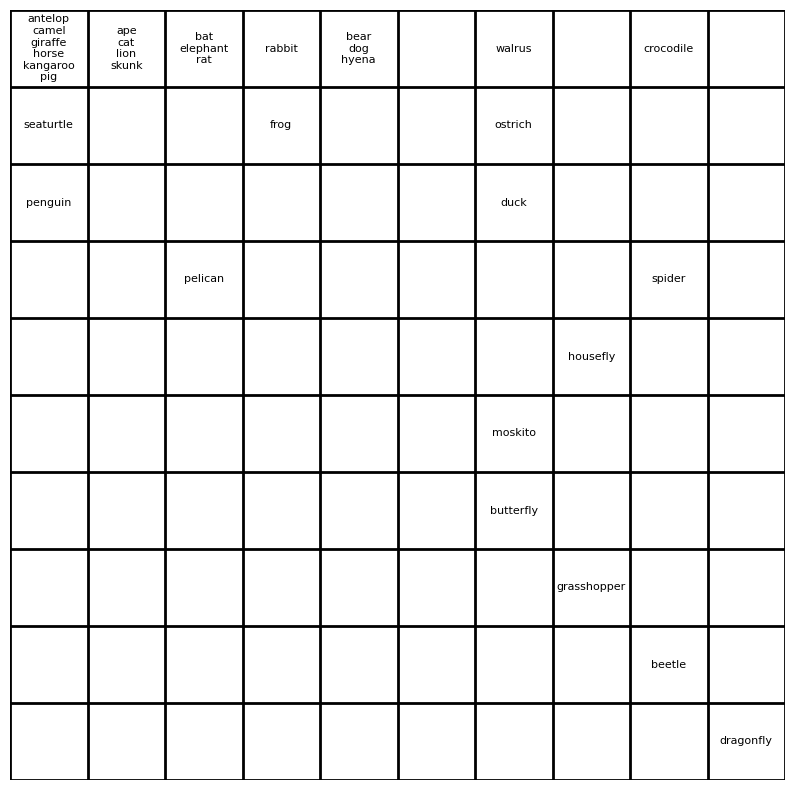
\includegraphics[width=5cm]{Labs/Lab 2/Results/animal_som.png}
    \caption{Animals sorted in 100 size nodes}
    \label{fig:SOM_animals}
\end{figure}
In the code we set the initial neighbors to 50, had 1000 epochs and a learning rate of 0.2 as in the instructions. The figure can be seen in \ref{fig:SOM_animals}. The figure makes sense as cat and lion are matched together and with closer observation you'll notice how most insects are grouped together. However they are certain places where it does not entirely make sense, specifically between frog, ape and walrus. In general it made sense. 



\subsection{Cyclic tour}
Figure \ref{fig:SOM_cycle} represents the shortest cycling tour which passes through all the cities based on their coordinates. 
\begin{figure}[htb]
    \centering
    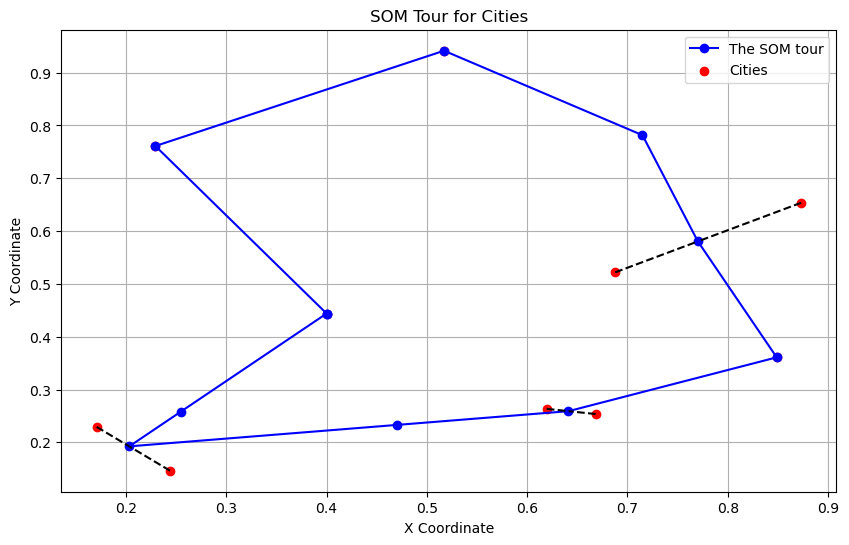
\includegraphics[width=7.5cm]{Labs/Lab 2/Results/Cyclic_som.png}
    \caption{Best path by SOM network}
    \label{fig:SOM_cycle}
\end{figure}

\subsection{Clustering with SOM}

\section{Final remarks \normalsize{\textit{(max 0.5 page)}}}
\textit{Please share your final reflections on the lab, its content and your own learning. Which parts of the lab assignment did you find confusing or not necessarily helping in understanding important concepts and which parts you have found interesting and relevant to your learning experience? \\
Here you can also formulate your opinion, interpretation or speculation about some of the simulation outcomes. Please add any follow-up questions that you might have regarding the lab tasks and the results you have produced.}

\end{document}
